\begin{frame}
	\myheading{Module 13.3 : Occlusion experiments}
\end{frame}

%%%%%%%%%%%%%%%%%%%%%%%%%%%%%%%%%%%%%%%%%%%%%%%%%%%%%%%%%%%%%%%%%%%%%%%%%%%%%%%%%%%%%%%%%

\begin{frame}
	\begin{columns}
		\column{0.5\textwidth}
		\begin{overlayarea}{\textwidth}{\textheight}
			% \only<1>{
			% 	\begin{figure}[hbtp]
			% 	\includegraphics[scale=0.15,trim={0cm 0cm 72cm 0cm}, clip=true]{img/s1_4_1.pdf}
			% 	\end{figure}
			% 	}
			% \only<2>{
			% 	\begin{figure}[hbtp]
			% 	\includegraphics[scale=0.15,trim={17.5cm 0cm 55cm 0cm}, clip=true]{img/s1_4_1.pdf}
			% 	\end{figure}
			% 	}
			\only<1->{
				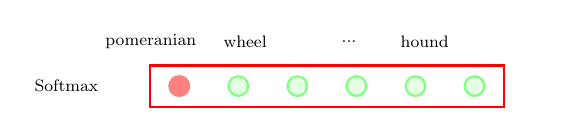
\begin{tikzpicture}[scale=0.75, transform shape]
	\tikzstyle{input_neuron}=[circle,draw=red!50,fill=red!10,thick,minimum size=2mm]
	\tikzstyle{hidden_neuron}=[circle,draw=blue!50,fill=cyan!10,thick,minimum size=2mm]
	\tikzstyle{output_neuron}=[circle,draw=green!50,fill=green!10,thick,minimum size=2mm]
	\tikzstyle{cpy_neuron}=[circle,draw=red!50,fill=red!50,thick,minimum size=2mm]
	\tikzstyle{input}=[circle,draw=black!50,fill=black!20,thick,minimum size=2mm]
	\node [text width = 7mm] at (10.9, 1.85){\footnotesize Softmax};
	\node [text width = 25mm] at (13,2.6){\footnotesize pomeranian};
	\node [text width = 25mm] at (15,2.6){\footnotesize wheel};
	\node [text width = 25mm] at (18,2.6){\footnotesize hound};
	\node [text width = 25mm] at (17,2.6){\footnotesize ...};
	\node [text width = 25mm] at (16,2.6){};
	\node [output_neuron] (neuron51) at (13,1.85) {};
	\node [output_neuron] (neuron51) at (17,1.85) {};
		
	\node [output_neuron] (neuron52) at (14,1.85)  {};
	\node [output_neuron] (neuron53) at (15,1.85)  {};
	\node [output_neuron] (neuron54) at (16,1.85)  {};
	\node [output_neuron] (neuron54) at (18,1.85)  {};
	\draw[red!100,thick,solid] (12.5,1.5) rectangle (18.5,2.2);
	\node [cpy_neuron] (neuron01) at (13,1.85) {};
\end{tikzpicture}
			}
			\vspace{-0.5cm}
			\only<1>{
				\begin{figure}
					\includegraphics[scale=0.1,trim={0cm 31.5cm 72cm 0cm}, clip=true]{images/s1_4_1.pdf}
				\end{figure}
			}
					
			\only<2>{
				\begin{figure}
					\includegraphics[scale=0.1,trim={0cm 31.5cm 55cm 0cm}, clip=true]{images/s1_4_1.pdf}
				\end{figure}
			}
			
			\only<3>{
				
				\begin{figure}
					\includegraphics[scale=0.1,trim={0cm 15.5cm 55cm 0cm}, clip=true]{images/s1_4_1.pdf}
				\end{figure}
			}
			
			\only<4>{
				
				\begin{figure}
					\includegraphics[scale=0.1,trim={0cm 0cm 55cm 0cm}, clip=true]{images/s1_4_1.pdf}
				\end{figure}
			}
		\end{overlayarea}
		\column{0.5\textwidth}
		\begin{overlayarea}{\textwidth}{\textheight}
			\begin{itemize}
				\justifying
				\item<1-> Typically we are interested in understanding which portions of the image are responsible 
				for maximizing the probability of a certain class
				\item<2-> We could occlude (gray out) different patches in the image and see the effect on the predicted probability of the correct class
				\item<3->For example this heat map shows that occluding the face of the dog causes a maximum drop in the prediction probability
				\item<4-> Similar observations are made for other images
			\end{itemize}
		\end{overlayarea}
	\end{columns}
	
\end{frame}